\documentclass[letterpaper,12pt]{article}

\usepackage{hyperref}
\RequirePackage{GE05}
% this inputs graphicx, too
\RequirePackage{comment}

\newcommand{\GDP}{\mbox{\em GDP\/}}
\newcommand{\NDP}{\mbox{\em NDP\/}}
\newcommand{\GNP}{\mbox{\em GNP\/}}
\newcommand{\NX}{\mbox{\em NX\/}}
\newcommand{\NY}{\mbox{\em NY\/}}
\newcommand{\CA}{\mbox{\em CA\/}}
\newcommand{\NFA}{\mbox{\em NFA\/}}
\newcommand{\Def}{\mbox{\em Def\/}}
\newcommand{\CPI}{\mbox{\em CPI\/}}
\newcommand{\phm}{\phantom{--}}

\def\ClassName{The Global Economy}
\def\Category{Professor David Backus}
\def\HeadName{Practice Midterm Exam}

\begin{document}
\parindent = 0.0in
\parskip = \bigskipamount
\thispagestyle{empty}%
\Head

\centerline{\large \bf \HeadName}%
\centerline{Revised:  \today}

\bigskip
You have 75 minutes to complete this exam.  Please answer each
question in the space provided. You may consult one page of notes
and a calculator, but devices capable of wireless transmission are
prohibited.

I understand that the honor code applies: I will not lie, cheat, or
steal to gain an academic advantage, or tolerate those who do.

\begin{flushright}
\rule{4in}{0.5pt} \\ (Name and Signature)
\end{flushright}


\bigskip
\begin{enumerate}

%\leftmargin=0.5in \labelwidth=\leftmargin
\begin{figure}[h]
    \centering
    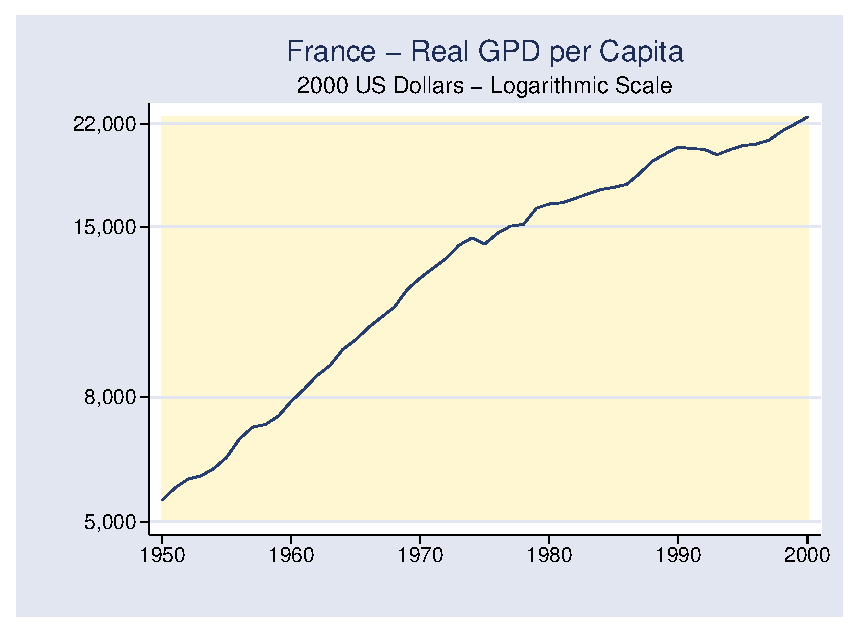
\includegraphics[scale=0.8]{france_gdp.eps}
    \caption{Economic Growth in France, 1950-2000.}
    \label{fig:france_gdp}
\end{figure}
%

\item {\it Economic growth in France.} Figure~\ref{fig:france_gdp}
depicts the path of France's GDP per capita in the period
1950-2000.
%\end{enumerate}
%\end{document}
%
The graph reveals that growth slowed down over this period. Your
task is to understand why. Here are some data that you will find
useful:
%
\begin{center}
%\tabcolsep = 0.12in
\begin{tabular}{lccccc}
\hline\hline
Year   &      GDP      &  Population  &  Capital    &  Labor   & Education  \\
\hline\hline
1961   &     387       &   47.317     & 1,110       & 20.410   &   5.44     \\%
1974   &     769       &   53.771     & 1,920       & 23.174   &   6.00     \\%
2000   &     1,350     &   60.431     & 3,850       & 27.497   &   7.86     \\%
\hline\hline
\end{tabular}
\end{center}
%
GDP and capital are expressed in billions of 2000 US dollars.
Population and employment are in millions of heads. Education is
the average number of years of school completed among people older
than 15.

\begin{enumerate}

\item Compute the (average continuously compounded) growth rates
of GDP per capita and GDP per worker over the period 1961-2000.
(10~points)

\item Use our growth accounting methodology to allocate growth in
output per capita over the period 1961-2000 to growth in TFP,
employment rate, capital per worker, and human capital,
respectively. What factors are most important? (10~points)

\item Now consider the sub-periods 1961-74 and 1975-2000 in
isolation. What are the main differences between the two? What may
have been the causes of such differences? (20~points)

\end{enumerate}


%\begin{comment}
Answer.  % ---------------------------------------------------------
\begin{enumerate}

\item The growth rate of GDP per capita is
$\log(22,339.53/8,178.88)/39 = 2.58\%$. Similarly, the growth rate
of GDP per worker is 2.44\%.

\item  The numbers are:
%
\begin{center}
%\tabcolsep = 0.12in
\begin{tabular}{lccccc}
\hline\hline
                                &     $Y/N$    &  $A$    &  $L/N$  & $K/L$    &  $H$   \\
\hline\hline
Growth Rate (\%)                &    2.58      &   1.00     &  0.14 & 2.42   & 0.94   \\
Contribution to GDP Growth (\%) &    2.58      &   1.00     &  0.14 & 0.81   & 0.63   \\
 \hline\hline
\end{tabular}
\end{center}
The most important factors, in order, are TFP, capital per worker,
and education.


\item Similar calculations for the two subperiods lead to:
%
\begin{center}
%\tabcolsep = 0.12in
\begin{tabular}{llccccc}
\hline\hline
Period       &                                 &     $Y/N$      &  $A$      &  $L/N$     & $K/L$    &  $H$   \\
\hline\hline
1961-74      & Growth Rate (\%)                &    4.30      &   2.72     &  0    & 3.24   & 0.75   \\
             & Contribution (\%) &    4.30      &   2.72     &  0    & 1.08   & 0.50   \\
1974-2000    & Growth Rate (\%)                &    1.71      &   0.14     &  0.21 & 2.02   & 1.04   \\
             & Contribution (\%) &    1.71      &   0.14     &  0.21 & 0.67   & 0.69   \\
\hline\hline
\end{tabular}
\end{center}
Apparently the big difference is the falloff in TFP growth.
You might ask yourself why.  My guess would be 
labor and production market frictions, which make the economy
less able to adapt to changes in the global business environment.  

\end{enumerate}
%\end{comment}


% ======================================================================
\item {\it The sorry state of fashion.} An
\href{http://www.economist.com/displaystory.cfm?story_id=3599862}{article}
in the January 27th issue of {\it The Economist\/} described the
troubles facing the textile industry in France and Italy. You
might read it for your own amusement.  We will use it simply to
motivate the following three imaginary statements, which are
inspired by (if not taken directly from) statements in the
article. For each of them, write down whether you agree or
disagree, and why.

\begin{enumerate}

\item Fran\c{c}ois Bertiet, who works as a driver for the group
Pinault-Printemps-Redoute, was recently interviewed by the TV
channel France 2. He argued that tariffs on Chinese clothing are
justified on the grounds that Chinese competition is unfair,
because it is driven by lower wages, rather than higher
productivity. (10~points)

\item Giuseppina Artioni, a retired public servant from Gallarate
and fashionable dresser, a town close to the infamous
Milan-Malpensa Airport, declared that the EU should keep its gates
wide open to Chinese clothing. What matters, she added, is that
European consumers can buy clothes cheaply. Foreign competition
insures just that. (10~points)

\item Jacqueline Hinault (unrelated to the famous cyclist Bernard
Hinault), a professor of fashion economics at the Universit\'{e}
du Tourmalet, recently argued in favor of free trade with China.
However, she added that the EU should force China to fight
counterfeiting. According to Professor Hinault, the inability to
enforce trademarks, by lowering the incentives for designers,
could lead to lower quality, just as counterfeiting of music CDs
is said to decrease the incentive to create music.  (10~points)

\end{enumerate}

%\begin{comment}
Answers.
\begin{enumerate}

\item We disagree with Monsieur Bertiet. If we buy foreign
clothing because it is less expensive, it makes no difference
whether it's cheap because it is produced by efficient workers or
by workers who are paid less than their French counterparts.
There's nothing ``unfair'' to Europeans about it. There's a sense
in which it's unfair to the Chinese --- certainly they'd like to
be paid more --- but that's a matter of their own productivity.
As long as their productivity is below European productivity,
their wages will be, too.

\item We agree with Signora Artioni.

\item We agree with Madame Hinault.  The idea behind intellectual
property protection (patents, copyrights, trademarks) is to give
the creator a monopoly right to the product as compensation for
the time and effort needed to develop it. In absence of such
protection, there is less incentive for people or companies to
develop and produce these products.  In the language of this
course, it's a case of having clear property rights.  There are
some differences between physical and intellectual property, but
that's a topic for another time.

\end{enumerate}
%\end{comment}


% ======================================================================
\item {\it Miscellany.}
%
\begin{enumerate}

\item The term \textit{off-shoring} has been coined to refer to
the relocation of work from one country (the US, say) to another
(India or China, for example).  What is the likely
\textit{short-run} effect of off-shoring US jobs to India on GDP,
Net Exports, and Net Factor Payments from Abroad for India and the
US? What is the likely \textit{long-run} effect on Indian and US
GDP? Why? (10~points)

\item A large domestic manufacturing company has asked Were \&
Very \& Cool, the consulting firm you work for, to advise it on
the location of a new plant. You are scheduled to give a
presentation to your team on labor market conditions in Lazystan,
one of the countries being considered by your client. On the IMF
web site you find that Lazystan's current population is 57m, of
which 10.3m are younger than 15 and 12.15m are older than 64. The
labor force is estimated to be 25 millions. The unemployment rate
is 10.17\%. In the introductory slide, you want to show the
absolute numbers of employed, unemployed, and inactive people,
along with employment rate, unemployment rate, and inactivity
rate. Please compute and report these figures. (10~points)

\item List two indicators that lead the business cycle in the US, 
and two that lag.  
(10~points)
\end{enumerate}


%\begin{comment}
Answers.
\begin{enumerate}

\item The answer to this question depends on the nature of goods
and services produced by US companies that relocate jobs to India.
Let us assume that they are final goods (and services).  In the
short run: US GDP probably falls, since it will take time for
other sectors of the economy to hire the workers whose jobs have
gone to India.  Net factor payments to the US probably rises, as
the US gets (say) the payments on capital invested abroad.  Net
Exports probably falls, because we're importing more from abroad.
In India you see the opposite:  GDP probably rises, factor
payments to India fall, and exports rise. In the long run:  GDP
increases in both the US and India through the
productivity-enhancing effects of trade.

Suppose, instead, that the ``off-shored'' goods and services are
intermediate rather than final goods.  Then there is also an
immediate positive effect on US value added, as cheaper prices of
intermediate goods trigger higher output of final goods.  In this
case, GDP may not fall even in the short run.  But it's asking a
lot for an answer.


\item The number of unemployed people is
$25,000,000\times.1017=2,542,500$. Therefore the number of
employed is $25,000,000-2,542,500=22,457,500$. The working-age
population is $57-10.3-12.15=34.55$ million. This implies that the
number of inactive is equal to $34.55-25=9.55$ million. The
employment rate is ${22,457,500}/{34,550,000}=65\%$. The
inactivity rate is ${9.55}/{34.55}=27.64\%$.

\item Leading indicators:  equity prices, long-short bond spread, 
hours worked in manufacturing.    
Lagging indicators:  employment, unemployment.  

\end{enumerate}
%\end{comment}

\end{enumerate}


\vfill \centerline{\it \copyright \ \number\year \ NYU Stern
School of Business}

%\end{document}

\pagebreak THE SORRY STATE OF FASHION TODAY Jan 27th 2005

From high fashion to the high street, Europe's rag trade is being
torn to shreds

THIS week Paris was abuzz with the biannual ritual of the city's
high-fashion shows. Giorgio Armani opened the series on January
24th, the Italian designer's first ever show in Paris. Almost
louder than the buzz of the shows, however, was the industry's
fretting over its own future. Europe's fashionistas are asking how
long high fashion can survive. With a dwindling client base and
copies rapidly available from clothes chains with quick production
cycles, it has become almost impossible to make money out of
custom-made garments.

Givenchy, Yves Saint Laurent, Versace and Valentino are all making
losses --- only Chanel is thought to make money. After failing to
make a profit for years, Ungaro is up for sale, and on January
25th Moet Hennessy Louis Vuitton (LVMH), a luxury-goods firm, sold
Christian Lacroix, another loss-making brand, to American
duty-free retailers for a ``symbolic" price. Prada has parted
company with Helmut Lang after persistent losses. Ten years ago,
more than 20 houses held Paris shows; today only a handful can
afford to carry on.

Europe's rag trade has been in trouble now for more than five
years. Luxury-goods groups reliant on glamorous names keep high
fashion alive. Valentino, for example, is owned by Marzotto,
Italy's biggest clothing and textile group; Yves Saint Laurent
belongs to Pinault-Printemps-Redoute, a French rival to LVMH.

Further down the fashion chain things are equally dire.
Mass-market producers cannot afford sustained losses. Medium-sized
and small companies in France, Italy and Spain are cutting
production or moving it abroad. Some have merged or tried to cut
costs by lowering the quality of their products. Dozens have
already gone under; many more are fighting for survival.

THE EFFECTS OF CHINA The main cause of the mass market's troubles
is competition from China. Producers cannot match its low labour
costs: the effect can be devastating, says Didier Grumbach at the
Federation Francaise de la Couture, France's main fashion
association.

And it can only get worse. Since January 1st world trade in
textiles has been freed of all restrictions, and members of the
European Union (EU) are expecting a flood of Chinese imports. At
the moment the EU is the world's leading exporter of textiles and
the second-largest exporter of clothing. The industry employed
2.7m people in 2003 and had a turnover of more than EURO225
billion (\$250 billion). But the EU's imports of Chinese textiles
and clothing almost doubled between 2001 and 2003, partly as a
result of a phase-out of quotas that began ten years ago. The
World Trade Organisation (WTO) predicts that within two years
China could control about 50\% of the world's textile market.

Home to more than half of Europe's textile companies, Italy stands
to suffer most from China's new freedom. It has some 50,000
textile companies clustered in Biella, Como and other regions.
They are small, often family-run firms employing an average of ten
people. Nearly two-thirds of their production is exported.

Many of these firms have already felt the pinch. Fratelli
Piacenza, a cashmere company in Biella, is moving production to
lower-wage countries. Other firms have reduced production and cut
workers. Yet more jobs will go this year. ``Italy is now going
through the crisis that happened in France about eight years ago,"
says Mario Boselli, boss of the Camera Nazionale della Moda,
Italy's big fashion association.

In France, dozens of firms went out of business between 1993 and
2003, when about one-third of the industry's jobs were lost. Today
more than 60\% of French brands are produced abroad. Kindy, a
sock-maker, started to move part of its production to North Africa
and Portugal in the
1990s. Now it is planning to produce even more cheaply by moving 30\% 
of its production to China over the next three years.

The French and Italian fashion associations have long been bitter
rivals, but on January 17th Messrs Grumbach and Boselli agreed on
a plan designed to soften the shock caused by the ending of
textile quotas. They intend to co-operate in the battle against
counterfeiting and to fight for further measures to stem the flow
of low-quality textile imports.

The industry's most effective lobby, however, is Euratex, a trade
association based in Brussels. Over the past few months it has
argued for ``safeguards", controversial instruments used to justify
stemming the flood of Chinese imports. Safeguards were built into
the agreement that America signed with China in November 1999 as
part of China's accession to the WTO. Turkey decided on January
9th to use safeguards on 43 categories of Chinese textiles, and
Argentina recently imposed similar quotas on textile imports from
China. Euratex is sure there will be a case for invoking
safeguards in the EU soon. In 2002 and 2003 imports of anoraks
from China increased three or four times while prices fell by
75\%, says a spokesman. (Quotas for anoraks ended earlier than
those for other products.)

Peter Mandelson, the EU trade commissioner, has so far been cold
towards the idea of re-imposing restrictions. The European
Commission says it is working on guidelines for the imposition of
safeguards, but it has been saying that for the last three months,
grumbles Thierry Noblot of the Union des Industries Textiles, the
French industry's main lobby group.

China is thinking of imposing restrictions itself: setting minimum
prices on some clothing exports in addition to export duties of 2-4\% on
some textiles. But neither measure is likely to have much effect.
European firms need to continue restructuring for the new textile
world, where they must focus on quality and innovation, their only
competitive advantages over China. Italy's Biella is spending
EURO2.8m on a marketing campaign to promote ``the art of
excellence".

The need for innovation and excellence is also the best argument
for the survival of Europe's haute couture. Now that Mr Armani has
at last been to the Paris shows, he must return again and again.

See this article with graphics and related items
\href{http://www.economist.com/displaystory.cfm?story_id=3599862}{here}.


\end{document}

Others:  
(i) Why u is less of a deal in France than L.  
(ii) Cycle question....  
(iii) Quant:  pop, emp, unemp, hours (France??) 


